% Options for packages loaded elsewhere
\PassOptionsToPackage{unicode}{hyperref}
\PassOptionsToPackage{hyphens}{url}
%
\documentclass[
]{article}
\usepackage{amsmath,amssymb}
\usepackage{lmodern}
\usepackage{ifxetex,ifluatex}
\ifnum 0\ifxetex 1\fi\ifluatex 1\fi=0 % if pdftex
  \usepackage[T1]{fontenc}
  \usepackage[utf8]{inputenc}
  \usepackage{textcomp} % provide euro and other symbols
\else % if luatex or xetex
  \usepackage{unicode-math}
  \defaultfontfeatures{Scale=MatchLowercase}
  \defaultfontfeatures[\rmfamily]{Ligatures=TeX,Scale=1}
\fi
% Use upquote if available, for straight quotes in verbatim environments
\IfFileExists{upquote.sty}{\usepackage{upquote}}{}
\IfFileExists{microtype.sty}{% use microtype if available
  \usepackage[]{microtype}
  \UseMicrotypeSet[protrusion]{basicmath} % disable protrusion for tt fonts
}{}
\makeatletter
\@ifundefined{KOMAClassName}{% if non-KOMA class
  \IfFileExists{parskip.sty}{%
    \usepackage{parskip}
  }{% else
    \setlength{\parindent}{0pt}
    \setlength{\parskip}{6pt plus 2pt minus 1pt}}
}{% if KOMA class
  \KOMAoptions{parskip=half}}
\makeatother
\usepackage{xcolor}
\IfFileExists{xurl.sty}{\usepackage{xurl}}{} % add URL line breaks if available
\IfFileExists{bookmark.sty}{\usepackage{bookmark}}{\usepackage{hyperref}}
\hypersetup{
  pdftitle={Class 09 Mini-Project Completed},
  pdfauthor={Claire Chapman},
  hidelinks,
  pdfcreator={LaTeX via pandoc}}
\urlstyle{same} % disable monospaced font for URLs
\usepackage[margin=1in]{geometry}
\usepackage{color}
\usepackage{fancyvrb}
\newcommand{\VerbBar}{|}
\newcommand{\VERB}{\Verb[commandchars=\\\{\}]}
\DefineVerbatimEnvironment{Highlighting}{Verbatim}{commandchars=\\\{\}}
% Add ',fontsize=\small' for more characters per line
\usepackage{framed}
\definecolor{shadecolor}{RGB}{248,248,248}
\newenvironment{Shaded}{\begin{snugshade}}{\end{snugshade}}
\newcommand{\AlertTok}[1]{\textcolor[rgb]{0.94,0.16,0.16}{#1}}
\newcommand{\AnnotationTok}[1]{\textcolor[rgb]{0.56,0.35,0.01}{\textbf{\textit{#1}}}}
\newcommand{\AttributeTok}[1]{\textcolor[rgb]{0.77,0.63,0.00}{#1}}
\newcommand{\BaseNTok}[1]{\textcolor[rgb]{0.00,0.00,0.81}{#1}}
\newcommand{\BuiltInTok}[1]{#1}
\newcommand{\CharTok}[1]{\textcolor[rgb]{0.31,0.60,0.02}{#1}}
\newcommand{\CommentTok}[1]{\textcolor[rgb]{0.56,0.35,0.01}{\textit{#1}}}
\newcommand{\CommentVarTok}[1]{\textcolor[rgb]{0.56,0.35,0.01}{\textbf{\textit{#1}}}}
\newcommand{\ConstantTok}[1]{\textcolor[rgb]{0.00,0.00,0.00}{#1}}
\newcommand{\ControlFlowTok}[1]{\textcolor[rgb]{0.13,0.29,0.53}{\textbf{#1}}}
\newcommand{\DataTypeTok}[1]{\textcolor[rgb]{0.13,0.29,0.53}{#1}}
\newcommand{\DecValTok}[1]{\textcolor[rgb]{0.00,0.00,0.81}{#1}}
\newcommand{\DocumentationTok}[1]{\textcolor[rgb]{0.56,0.35,0.01}{\textbf{\textit{#1}}}}
\newcommand{\ErrorTok}[1]{\textcolor[rgb]{0.64,0.00,0.00}{\textbf{#1}}}
\newcommand{\ExtensionTok}[1]{#1}
\newcommand{\FloatTok}[1]{\textcolor[rgb]{0.00,0.00,0.81}{#1}}
\newcommand{\FunctionTok}[1]{\textcolor[rgb]{0.00,0.00,0.00}{#1}}
\newcommand{\ImportTok}[1]{#1}
\newcommand{\InformationTok}[1]{\textcolor[rgb]{0.56,0.35,0.01}{\textbf{\textit{#1}}}}
\newcommand{\KeywordTok}[1]{\textcolor[rgb]{0.13,0.29,0.53}{\textbf{#1}}}
\newcommand{\NormalTok}[1]{#1}
\newcommand{\OperatorTok}[1]{\textcolor[rgb]{0.81,0.36,0.00}{\textbf{#1}}}
\newcommand{\OtherTok}[1]{\textcolor[rgb]{0.56,0.35,0.01}{#1}}
\newcommand{\PreprocessorTok}[1]{\textcolor[rgb]{0.56,0.35,0.01}{\textit{#1}}}
\newcommand{\RegionMarkerTok}[1]{#1}
\newcommand{\SpecialCharTok}[1]{\textcolor[rgb]{0.00,0.00,0.00}{#1}}
\newcommand{\SpecialStringTok}[1]{\textcolor[rgb]{0.31,0.60,0.02}{#1}}
\newcommand{\StringTok}[1]{\textcolor[rgb]{0.31,0.60,0.02}{#1}}
\newcommand{\VariableTok}[1]{\textcolor[rgb]{0.00,0.00,0.00}{#1}}
\newcommand{\VerbatimStringTok}[1]{\textcolor[rgb]{0.31,0.60,0.02}{#1}}
\newcommand{\WarningTok}[1]{\textcolor[rgb]{0.56,0.35,0.01}{\textbf{\textit{#1}}}}
\usepackage{graphicx}
\makeatletter
\def\maxwidth{\ifdim\Gin@nat@width>\linewidth\linewidth\else\Gin@nat@width\fi}
\def\maxheight{\ifdim\Gin@nat@height>\textheight\textheight\else\Gin@nat@height\fi}
\makeatother
% Scale images if necessary, so that they will not overflow the page
% margins by default, and it is still possible to overwrite the defaults
% using explicit options in \includegraphics[width, height, ...]{}
\setkeys{Gin}{width=\maxwidth,height=\maxheight,keepaspectratio}
% Set default figure placement to htbp
\makeatletter
\def\fps@figure{htbp}
\makeatother
\setlength{\emergencystretch}{3em} % prevent overfull lines
\providecommand{\tightlist}{%
  \setlength{\itemsep}{0pt}\setlength{\parskip}{0pt}}
\setcounter{secnumdepth}{-\maxdimen} % remove section numbering
\ifluatex
  \usepackage{selnolig}  % disable illegal ligatures
\fi

\title{Class 09 Mini-Project Completed}
\author{Claire Chapman}
\date{10/29/2021}

\begin{document}
\maketitle

\hypertarget{preparing-the-data}{%
\subsection{Preparing the Data}\label{preparing-the-data}}

Reading in the data

\begin{Shaded}
\begin{Highlighting}[]
\NormalTok{fna.data }\OtherTok{\textless{}{-}} \StringTok{"WisconsinCancer.csv"}
\NormalTok{wisc.df }\OtherTok{\textless{}{-}} \FunctionTok{read.csv}\NormalTok{(fna.data, }\AttributeTok{row.names =} \DecValTok{1}\NormalTok{)}
\end{Highlighting}
\end{Shaded}

Examine the data

\begin{Shaded}
\begin{Highlighting}[]
\FunctionTok{head}\NormalTok{(wisc.df)}
\end{Highlighting}
\end{Shaded}

\begin{verbatim}
##          diagnosis radius_mean texture_mean perimeter_mean area_mean
## 842302           M       17.99        10.38         122.80    1001.0
## 842517           M       20.57        17.77         132.90    1326.0
## 84300903         M       19.69        21.25         130.00    1203.0
## 84348301         M       11.42        20.38          77.58     386.1
## 84358402         M       20.29        14.34         135.10    1297.0
## 843786           M       12.45        15.70          82.57     477.1
##          smoothness_mean compactness_mean concavity_mean concave.points_mean
## 842302           0.11840          0.27760         0.3001             0.14710
## 842517           0.08474          0.07864         0.0869             0.07017
## 84300903         0.10960          0.15990         0.1974             0.12790
## 84348301         0.14250          0.28390         0.2414             0.10520
## 84358402         0.10030          0.13280         0.1980             0.10430
## 843786           0.12780          0.17000         0.1578             0.08089
##          symmetry_mean fractal_dimension_mean radius_se texture_se perimeter_se
## 842302          0.2419                0.07871    1.0950     0.9053        8.589
## 842517          0.1812                0.05667    0.5435     0.7339        3.398
## 84300903        0.2069                0.05999    0.7456     0.7869        4.585
## 84348301        0.2597                0.09744    0.4956     1.1560        3.445
## 84358402        0.1809                0.05883    0.7572     0.7813        5.438
## 843786          0.2087                0.07613    0.3345     0.8902        2.217
##          area_se smoothness_se compactness_se concavity_se concave.points_se
## 842302    153.40      0.006399        0.04904      0.05373           0.01587
## 842517     74.08      0.005225        0.01308      0.01860           0.01340
## 84300903   94.03      0.006150        0.04006      0.03832           0.02058
## 84348301   27.23      0.009110        0.07458      0.05661           0.01867
## 84358402   94.44      0.011490        0.02461      0.05688           0.01885
## 843786     27.19      0.007510        0.03345      0.03672           0.01137
##          symmetry_se fractal_dimension_se radius_worst texture_worst
## 842302       0.03003             0.006193        25.38         17.33
## 842517       0.01389             0.003532        24.99         23.41
## 84300903     0.02250             0.004571        23.57         25.53
## 84348301     0.05963             0.009208        14.91         26.50
## 84358402     0.01756             0.005115        22.54         16.67
## 843786       0.02165             0.005082        15.47         23.75
##          perimeter_worst area_worst smoothness_worst compactness_worst
## 842302            184.60     2019.0           0.1622            0.6656
## 842517            158.80     1956.0           0.1238            0.1866
## 84300903          152.50     1709.0           0.1444            0.4245
## 84348301           98.87      567.7           0.2098            0.8663
## 84358402          152.20     1575.0           0.1374            0.2050
## 843786            103.40      741.6           0.1791            0.5249
##          concavity_worst concave.points_worst symmetry_worst
## 842302            0.7119               0.2654         0.4601
## 842517            0.2416               0.1860         0.2750
## 84300903          0.4504               0.2430         0.3613
## 84348301          0.6869               0.2575         0.6638
## 84358402          0.4000               0.1625         0.2364
## 843786            0.5355               0.1741         0.3985
##          fractal_dimension_worst
## 842302                   0.11890
## 842517                   0.08902
## 84300903                 0.08758
## 84348301                 0.17300
## 84358402                 0.07678
## 843786                   0.12440
\end{verbatim}

Get rid of the ``Diagnosis'' column because we won't be needing it

\begin{Shaded}
\begin{Highlighting}[]
\NormalTok{wisc.data }\OtherTok{\textless{}{-}}\NormalTok{ wisc.df[,}\SpecialCharTok{{-}}\DecValTok{1}\NormalTok{]}
\end{Highlighting}
\end{Shaded}

But store ``Diagnosis'' as a factor to be used later to check our work

\begin{Shaded}
\begin{Highlighting}[]
\NormalTok{diagnosis }\OtherTok{\textless{}{-}} \FunctionTok{as.factor}\NormalTok{(wisc.df}\SpecialCharTok{$}\NormalTok{diagnosis)}
\end{Highlighting}
\end{Shaded}

\begin{quote}
Q1. How many observations are in this dataset?
\end{quote}

\begin{Shaded}
\begin{Highlighting}[]
\FunctionTok{dim}\NormalTok{(wisc.data)}
\end{Highlighting}
\end{Shaded}

\begin{verbatim}
## [1] 569  30
\end{verbatim}

569 observations

\begin{quote}
Q2. How many of the observations have a malignant diagnosis?
\end{quote}

\begin{Shaded}
\begin{Highlighting}[]
\FunctionTok{table}\NormalTok{(diagnosis)}
\end{Highlighting}
\end{Shaded}

\begin{verbatim}
## diagnosis
##   B   M 
## 357 212
\end{verbatim}

\begin{quote}
Q3. How many variables/features in the data are suffixed with \_mean?
\end{quote}

\begin{Shaded}
\begin{Highlighting}[]
\FunctionTok{length}\NormalTok{(}\FunctionTok{grep}\NormalTok{(}\StringTok{"\_mean"}\NormalTok{, }\FunctionTok{colnames}\NormalTok{(wisc.data)))}
\end{Highlighting}
\end{Shaded}

\begin{verbatim}
## [1] 10
\end{verbatim}

\hypertarget{principal-component-analysis}{%
\subsection{Principal Component
Analysis}\label{principal-component-analysis}}

Checking column means and standard deviation

\begin{Shaded}
\begin{Highlighting}[]
\FunctionTok{colMeans}\NormalTok{(wisc.data)}
\end{Highlighting}
\end{Shaded}

\begin{verbatim}
##             radius_mean            texture_mean          perimeter_mean 
##            1.412729e+01            1.928965e+01            9.196903e+01 
##               area_mean         smoothness_mean        compactness_mean 
##            6.548891e+02            9.636028e-02            1.043410e-01 
##          concavity_mean     concave.points_mean           symmetry_mean 
##            8.879932e-02            4.891915e-02            1.811619e-01 
##  fractal_dimension_mean               radius_se              texture_se 
##            6.279761e-02            4.051721e-01            1.216853e+00 
##            perimeter_se                 area_se           smoothness_se 
##            2.866059e+00            4.033708e+01            7.040979e-03 
##          compactness_se            concavity_se       concave.points_se 
##            2.547814e-02            3.189372e-02            1.179614e-02 
##             symmetry_se    fractal_dimension_se            radius_worst 
##            2.054230e-02            3.794904e-03            1.626919e+01 
##           texture_worst         perimeter_worst              area_worst 
##            2.567722e+01            1.072612e+02            8.805831e+02 
##        smoothness_worst       compactness_worst         concavity_worst 
##            1.323686e-01            2.542650e-01            2.721885e-01 
##    concave.points_worst          symmetry_worst fractal_dimension_worst 
##            1.146062e-01            2.900756e-01            8.394582e-02
\end{verbatim}

\begin{Shaded}
\begin{Highlighting}[]
\FunctionTok{apply}\NormalTok{(wisc.data, }\DecValTok{2}\NormalTok{, sd)}
\end{Highlighting}
\end{Shaded}

\begin{verbatim}
##             radius_mean            texture_mean          perimeter_mean 
##            3.524049e+00            4.301036e+00            2.429898e+01 
##               area_mean         smoothness_mean        compactness_mean 
##            3.519141e+02            1.406413e-02            5.281276e-02 
##          concavity_mean     concave.points_mean           symmetry_mean 
##            7.971981e-02            3.880284e-02            2.741428e-02 
##  fractal_dimension_mean               radius_se              texture_se 
##            7.060363e-03            2.773127e-01            5.516484e-01 
##            perimeter_se                 area_se           smoothness_se 
##            2.021855e+00            4.549101e+01            3.002518e-03 
##          compactness_se            concavity_se       concave.points_se 
##            1.790818e-02            3.018606e-02            6.170285e-03 
##             symmetry_se    fractal_dimension_se            radius_worst 
##            8.266372e-03            2.646071e-03            4.833242e+00 
##           texture_worst         perimeter_worst              area_worst 
##            6.146258e+00            3.360254e+01            5.693570e+02 
##        smoothness_worst       compactness_worst         concavity_worst 
##            2.283243e-02            1.573365e-01            2.086243e-01 
##    concave.points_worst          symmetry_worst fractal_dimension_worst 
##            6.573234e-02            6.186747e-02            1.806127e-02
\end{verbatim}

Perform PCA

\begin{Shaded}
\begin{Highlighting}[]
\NormalTok{wisc.pr }\OtherTok{\textless{}{-}} \FunctionTok{prcomp}\NormalTok{(wisc.data, }\AttributeTok{scale =}\NormalTok{ T)}
\end{Highlighting}
\end{Shaded}

\begin{Shaded}
\begin{Highlighting}[]
\FunctionTok{summary}\NormalTok{(wisc.pr)}
\end{Highlighting}
\end{Shaded}

\begin{verbatim}
## Importance of components:
##                           PC1    PC2     PC3     PC4     PC5     PC6     PC7
## Standard deviation     3.6444 2.3857 1.67867 1.40735 1.28403 1.09880 0.82172
## Proportion of Variance 0.4427 0.1897 0.09393 0.06602 0.05496 0.04025 0.02251
## Cumulative Proportion  0.4427 0.6324 0.72636 0.79239 0.84734 0.88759 0.91010
##                            PC8    PC9    PC10   PC11    PC12    PC13    PC14
## Standard deviation     0.69037 0.6457 0.59219 0.5421 0.51104 0.49128 0.39624
## Proportion of Variance 0.01589 0.0139 0.01169 0.0098 0.00871 0.00805 0.00523
## Cumulative Proportion  0.92598 0.9399 0.95157 0.9614 0.97007 0.97812 0.98335
##                           PC15    PC16    PC17    PC18    PC19    PC20   PC21
## Standard deviation     0.30681 0.28260 0.24372 0.22939 0.22244 0.17652 0.1731
## Proportion of Variance 0.00314 0.00266 0.00198 0.00175 0.00165 0.00104 0.0010
## Cumulative Proportion  0.98649 0.98915 0.99113 0.99288 0.99453 0.99557 0.9966
##                           PC22    PC23   PC24    PC25    PC26    PC27    PC28
## Standard deviation     0.16565 0.15602 0.1344 0.12442 0.09043 0.08307 0.03987
## Proportion of Variance 0.00091 0.00081 0.0006 0.00052 0.00027 0.00023 0.00005
## Cumulative Proportion  0.99749 0.99830 0.9989 0.99942 0.99969 0.99992 0.99997
##                           PC29    PC30
## Standard deviation     0.02736 0.01153
## Proportion of Variance 0.00002 0.00000
## Cumulative Proportion  1.00000 1.00000
\end{verbatim}

\begin{quote}
Q4. From your results, what proportion of the original variance is
captured by the first principal components (PC1)?
\end{quote}

From row 2 of the summary above, PC1 accounts for 44.27\%

\begin{quote}
Q5. How many principal components (PCs) are required to describe at
least 70\% of the original variance in the data?
\end{quote}

From row 3 of the summary above, 3 PCs are required to describe
\textgreater70\%

\begin{quote}
Q6. How many principal components (PCs) are required to describe at
least 90\% of the original variance in the data?
\end{quote}

From row 3 of the summary above, 7 PCs are required to describe
\textgreater90\%

\hypertarget{interpreting-pca-results}{%
\subsection{Interpreting PCA Results}\label{interpreting-pca-results}}

\begin{Shaded}
\begin{Highlighting}[]
\FunctionTok{biplot}\NormalTok{(wisc.pr)}
\end{Highlighting}
\end{Shaded}

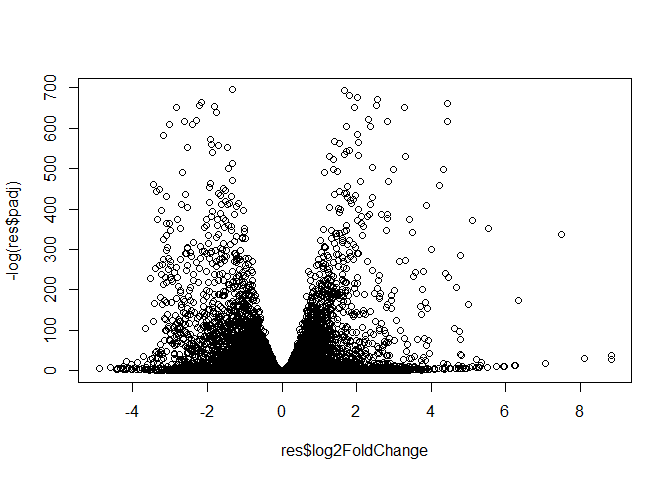
\includegraphics{Class09_files/figure-latex/unnamed-chunk-11-1.pdf}
\textgreater{} Q7. What stands out to you about this plot? Is it easy or
difficult to understand? Why?

There is way too much information on this plot for it to be understood
and to be useful.

Let's make a better plot

\begin{Shaded}
\begin{Highlighting}[]
\FunctionTok{plot}\NormalTok{(wisc.pr}\SpecialCharTok{$}\NormalTok{x[,}\DecValTok{1}\NormalTok{], wisc.pr}\SpecialCharTok{$}\NormalTok{x[,}\DecValTok{2}\NormalTok{], }\AttributeTok{col =}\NormalTok{ diagnosis, }\AttributeTok{xlab =} \StringTok{"PC1"}\NormalTok{, }\AttributeTok{ylab =} \StringTok{"PC2"}\NormalTok{)}
\end{Highlighting}
\end{Shaded}

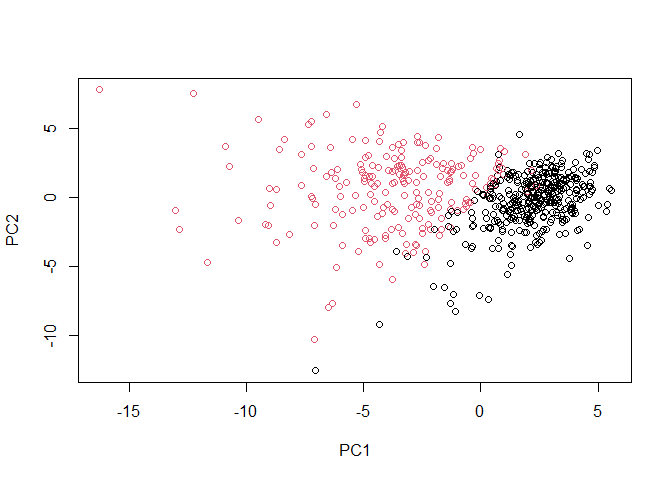
\includegraphics{Class09_files/figure-latex/unnamed-chunk-12-1.pdf}
\textgreater{} Q8. Generate a similar plot for principal components 1
and 3. What do you notice about these plots?

\begin{Shaded}
\begin{Highlighting}[]
\FunctionTok{plot}\NormalTok{(wisc.pr}\SpecialCharTok{$}\NormalTok{x[,}\DecValTok{1}\NormalTok{], wisc.pr}\SpecialCharTok{$}\NormalTok{x[,}\DecValTok{3}\NormalTok{], }\AttributeTok{col =}\NormalTok{ diagnosis, }\AttributeTok{xlab =} \StringTok{"PC1"}\NormalTok{, }\AttributeTok{ylab =} \StringTok{"PC3"}\NormalTok{)}
\end{Highlighting}
\end{Shaded}

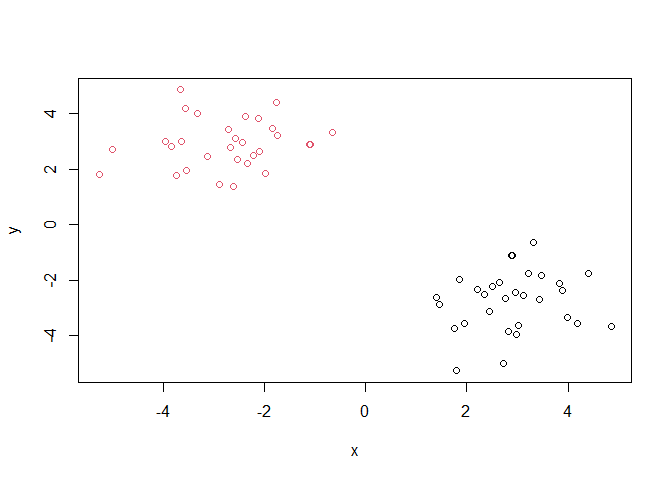
\includegraphics{Class09_files/figure-latex/unnamed-chunk-13-1.pdf}
\#\#\# Using ggplot2 to make another plot Turn the PCA into a dataframe,
add back diagnosis as a column

\begin{Shaded}
\begin{Highlighting}[]
\NormalTok{df }\OtherTok{\textless{}{-}} \FunctionTok{as.data.frame}\NormalTok{(wisc.pr}\SpecialCharTok{$}\NormalTok{x)}
\NormalTok{df}\SpecialCharTok{$}\NormalTok{diagnosis }\OtherTok{\textless{}{-}}\NormalTok{ diagnosis}
\end{Highlighting}
\end{Shaded}

\begin{Shaded}
\begin{Highlighting}[]
\FunctionTok{library}\NormalTok{(ggplot2)}
\end{Highlighting}
\end{Shaded}

Make a scatter plot colored by diagnosis

\begin{Shaded}
\begin{Highlighting}[]
\FunctionTok{ggplot}\NormalTok{(df, }\FunctionTok{aes}\NormalTok{(PC1, PC2, }\AttributeTok{col =}\NormalTok{ diagnosis)) }\SpecialCharTok{+}
  \FunctionTok{geom\_point}\NormalTok{()}
\end{Highlighting}
\end{Shaded}

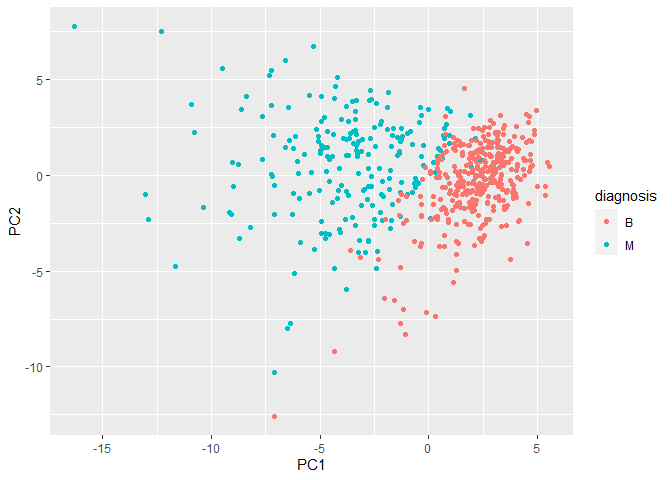
\includegraphics{Class09_files/figure-latex/unnamed-chunk-16-1.pdf}

\hypertarget{variance-explained}{%
\subsection{Variance Explained}\label{variance-explained}}

Calculate variance of each component

\begin{Shaded}
\begin{Highlighting}[]
\NormalTok{pr.var }\OtherTok{\textless{}{-}}\NormalTok{ wisc.pr}\SpecialCharTok{$}\NormalTok{sdev}\SpecialCharTok{\^{}}\DecValTok{2}
\FunctionTok{head}\NormalTok{(pr.var)}
\end{Highlighting}
\end{Shaded}

\begin{verbatim}
## [1] 13.281608  5.691355  2.817949  1.980640  1.648731  1.207357
\end{verbatim}

Calculate the variance explained by each principal component

\begin{Shaded}
\begin{Highlighting}[]
\NormalTok{pve }\OtherTok{\textless{}{-}}\NormalTok{ pr.var }\SpecialCharTok{/} \FunctionTok{sum}\NormalTok{(pr.var)}
\end{Highlighting}
\end{Shaded}

Plot variance explained for each principal component

\begin{Shaded}
\begin{Highlighting}[]
\FunctionTok{plot}\NormalTok{(pve, }\AttributeTok{xlab =} \StringTok{"Principal Component"}\NormalTok{, }\AttributeTok{ylab =} \StringTok{"Proportion of Variance Explained"}\NormalTok{, }\AttributeTok{ylim =} \FunctionTok{c}\NormalTok{(}\DecValTok{0}\NormalTok{,}\DecValTok{1}\NormalTok{), }\AttributeTok{type =} \StringTok{"o"}\NormalTok{)}
\end{Highlighting}
\end{Shaded}

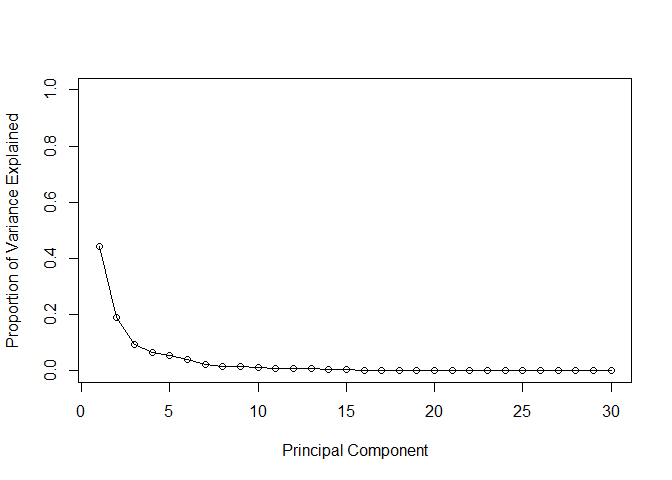
\includegraphics{Class09_files/figure-latex/unnamed-chunk-19-1.pdf}

Alternative scree plot of the same data

\begin{Shaded}
\begin{Highlighting}[]
\FunctionTok{barplot}\NormalTok{(pve, }\AttributeTok{ylab =} \StringTok{"Precent of Variance Explained"}\NormalTok{, }\AttributeTok{names.arg=}\FunctionTok{paste0}\NormalTok{(}\StringTok{"PC"}\NormalTok{,}\DecValTok{1}\SpecialCharTok{:}\FunctionTok{length}\NormalTok{(pve)), }\AttributeTok{las=}\DecValTok{2}\NormalTok{, }\AttributeTok{axes =} \ConstantTok{FALSE}\NormalTok{)}
\FunctionTok{axis}\NormalTok{(}\DecValTok{2}\NormalTok{, }\AttributeTok{at=}\NormalTok{pve, }\AttributeTok{labels=}\FunctionTok{round}\NormalTok{(pve,}\DecValTok{2}\NormalTok{)}\SpecialCharTok{*}\DecValTok{100}\NormalTok{ )}
\end{Highlighting}
\end{Shaded}

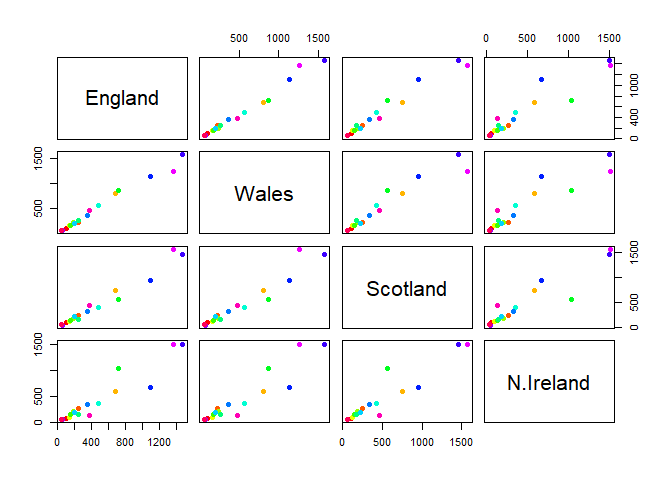
\includegraphics{Class09_files/figure-latex/unnamed-chunk-20-1.pdf}

\hypertarget{exploring-additional-cran-packages}{%
\subsubsection{Exploring additional CRAN
packages}\label{exploring-additional-cran-packages}}

\begin{Shaded}
\begin{Highlighting}[]
\CommentTok{\#install.packages("factoextra")}
\FunctionTok{library}\NormalTok{(factoextra)}
\end{Highlighting}
\end{Shaded}

\begin{verbatim}
## Welcome! Want to learn more? See two factoextra-related books at https://goo.gl/ve3WBa
\end{verbatim}

\begin{Shaded}
\begin{Highlighting}[]
\FunctionTok{fviz\_eig}\NormalTok{(wisc.pr, }\AttributeTok{addlabels =} \ConstantTok{TRUE}\NormalTok{)}
\end{Highlighting}
\end{Shaded}

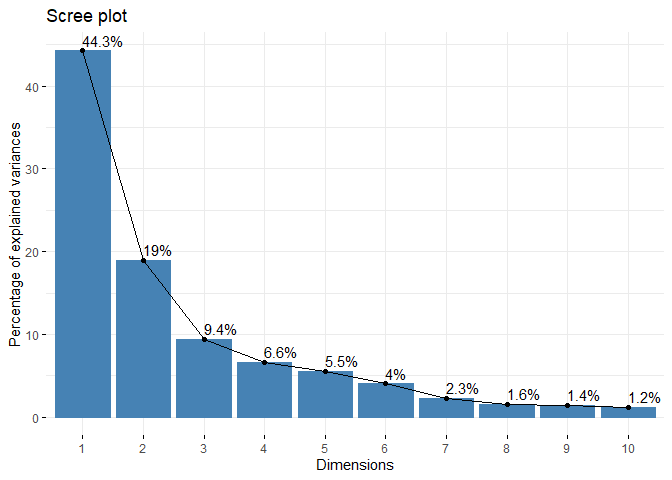
\includegraphics{Class09_files/figure-latex/unnamed-chunk-21-1.pdf}

\hypertarget{communicating-pca-results}{%
\subsection{Communicating PCA Results}\label{communicating-pca-results}}

Loadings: vectors that explain the mapping from the original features to
the PC

\begin{quote}
Q9. For the first principal component, what is the component of the
loading vector (i.e.~wisc.pr\$rotation{[},1{]}) for the feature
concave.points\_mean?
\end{quote}

\begin{Shaded}
\begin{Highlighting}[]
\NormalTok{wisc.pr}\SpecialCharTok{$}\NormalTok{rotation[,}\DecValTok{1}\NormalTok{]}
\end{Highlighting}
\end{Shaded}

\begin{verbatim}
##             radius_mean            texture_mean          perimeter_mean 
##             -0.21890244             -0.10372458             -0.22753729 
##               area_mean         smoothness_mean        compactness_mean 
##             -0.22099499             -0.14258969             -0.23928535 
##          concavity_mean     concave.points_mean           symmetry_mean 
##             -0.25840048             -0.26085376             -0.13816696 
##  fractal_dimension_mean               radius_se              texture_se 
##             -0.06436335             -0.20597878             -0.01742803 
##            perimeter_se                 area_se           smoothness_se 
##             -0.21132592             -0.20286964             -0.01453145 
##          compactness_se            concavity_se       concave.points_se 
##             -0.17039345             -0.15358979             -0.18341740 
##             symmetry_se    fractal_dimension_se            radius_worst 
##             -0.04249842             -0.10256832             -0.22799663 
##           texture_worst         perimeter_worst              area_worst 
##             -0.10446933             -0.23663968             -0.22487053 
##        smoothness_worst       compactness_worst         concavity_worst 
##             -0.12795256             -0.21009588             -0.22876753 
##    concave.points_worst          symmetry_worst fractal_dimension_worst 
##             -0.25088597             -0.12290456             -0.13178394
\end{verbatim}

The loading vector for concave.points\_mean is -0.260

\begin{quote}
Q10. What is the minimum number of principal components required to
explain 80\% of the variance of the data?
\end{quote}

\begin{Shaded}
\begin{Highlighting}[]
\FunctionTok{summary}\NormalTok{(wisc.pr)}
\end{Highlighting}
\end{Shaded}

\begin{verbatim}
## Importance of components:
##                           PC1    PC2     PC3     PC4     PC5     PC6     PC7
## Standard deviation     3.6444 2.3857 1.67867 1.40735 1.28403 1.09880 0.82172
## Proportion of Variance 0.4427 0.1897 0.09393 0.06602 0.05496 0.04025 0.02251
## Cumulative Proportion  0.4427 0.6324 0.72636 0.79239 0.84734 0.88759 0.91010
##                            PC8    PC9    PC10   PC11    PC12    PC13    PC14
## Standard deviation     0.69037 0.6457 0.59219 0.5421 0.51104 0.49128 0.39624
## Proportion of Variance 0.01589 0.0139 0.01169 0.0098 0.00871 0.00805 0.00523
## Cumulative Proportion  0.92598 0.9399 0.95157 0.9614 0.97007 0.97812 0.98335
##                           PC15    PC16    PC17    PC18    PC19    PC20   PC21
## Standard deviation     0.30681 0.28260 0.24372 0.22939 0.22244 0.17652 0.1731
## Proportion of Variance 0.00314 0.00266 0.00198 0.00175 0.00165 0.00104 0.0010
## Cumulative Proportion  0.98649 0.98915 0.99113 0.99288 0.99453 0.99557 0.9966
##                           PC22    PC23   PC24    PC25    PC26    PC27    PC28
## Standard deviation     0.16565 0.15602 0.1344 0.12442 0.09043 0.08307 0.03987
## Proportion of Variance 0.00091 0.00081 0.0006 0.00052 0.00027 0.00023 0.00005
## Cumulative Proportion  0.99749 0.99830 0.9989 0.99942 0.99969 0.99992 0.99997
##                           PC29    PC30
## Standard deviation     0.02736 0.01153
## Proportion of Variance 0.00002 0.00000
## Cumulative Proportion  1.00000 1.00000
\end{verbatim}

You need 5 principal components to explain \textgreater80\% of the
variance

\hypertarget{hierarchical-clustering}{%
\subsection{Hierarchical Clustering}\label{hierarchical-clustering}}

First scale the data

\begin{Shaded}
\begin{Highlighting}[]
\NormalTok{data.scaled }\OtherTok{\textless{}{-}} \FunctionTok{scale}\NormalTok{(wisc.data)}
\end{Highlighting}
\end{Shaded}

Calculate the distances between all pairs of observations

\begin{Shaded}
\begin{Highlighting}[]
\NormalTok{data.dist }\OtherTok{\textless{}{-}} \FunctionTok{dist}\NormalTok{(data.scaled)}
\end{Highlighting}
\end{Shaded}

Create hierarchical clustering model

\begin{Shaded}
\begin{Highlighting}[]
\NormalTok{wisc.hclust }\OtherTok{\textless{}{-}} \FunctionTok{hclust}\NormalTok{(data.dist, }\AttributeTok{method =} \StringTok{"complete"}\NormalTok{)}
\end{Highlighting}
\end{Shaded}

\hypertarget{results-of-hclustering}{%
\subsection{Results of HClustering}\label{results-of-hclustering}}

\begin{quote}
Q11. Using the plot() and abline() functions, what is the height at
which the clustering model has 4 clusters?
\end{quote}

\begin{Shaded}
\begin{Highlighting}[]
\FunctionTok{plot}\NormalTok{(wisc.hclust)}
\FunctionTok{abline}\NormalTok{(}\AttributeTok{h =} \DecValTok{19}\NormalTok{, }\AttributeTok{col =} \StringTok{"red"}\NormalTok{, }\AttributeTok{lty =} \DecValTok{2}\NormalTok{)}
\end{Highlighting}
\end{Shaded}

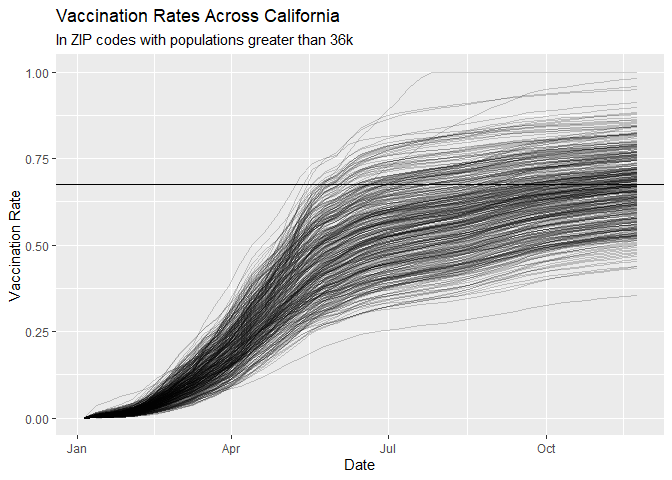
\includegraphics{Class09_files/figure-latex/unnamed-chunk-27-1.pdf}
There are four clusters at about height 19

\hypertarget{selecting-number-of-clusters}{%
\subsection{Selecting number of
clusters}\label{selecting-number-of-clusters}}

\begin{Shaded}
\begin{Highlighting}[]
\NormalTok{wisc.hclust.clusters }\OtherTok{\textless{}{-}} \FunctionTok{cutree}\NormalTok{(wisc.hclust, }\AttributeTok{h =} \DecValTok{19}\NormalTok{)}
\end{Highlighting}
\end{Shaded}

\begin{Shaded}
\begin{Highlighting}[]
\FunctionTok{table}\NormalTok{(wisc.hclust.clusters, diagnosis)}
\end{Highlighting}
\end{Shaded}

\begin{verbatim}
##                     diagnosis
## wisc.hclust.clusters   B   M
##                    1  12 165
##                    2   2   5
##                    3 343  40
##                    4   0   2
\end{verbatim}

\begin{quote}
Q12. Can you find a better cluster vs diagnoses match by cutting into a
different number of clusters between 2 and 10?
\end{quote}

\begin{Shaded}
\begin{Highlighting}[]
\NormalTok{wisc.xclusters }\OtherTok{\textless{}{-}} \FunctionTok{cutree}\NormalTok{(wisc.hclust, }\AttributeTok{h =} \DecValTok{13}\NormalTok{)}
\FunctionTok{table}\NormalTok{(wisc.xclusters, diagnosis)}
\end{Highlighting}
\end{Shaded}

\begin{verbatim}
##               diagnosis
## wisc.xclusters   B   M
##             1   12  86
##             2    0  59
##             3    0   3
##             4  331  39
##             5    0  20
##             6    2   0
##             7   12   0
##             8    0   2
##             9    0   2
##             10   0   1
\end{verbatim}

\begin{Shaded}
\begin{Highlighting}[]
\NormalTok{wisc.xclusters }\OtherTok{\textless{}{-}} \FunctionTok{cutree}\NormalTok{(wisc.hclust, }\AttributeTok{h =} \DecValTok{15}\NormalTok{)}
\FunctionTok{table}\NormalTok{(wisc.xclusters, diagnosis)}
\end{Highlighting}
\end{Shaded}

\begin{verbatim}
##               diagnosis
## wisc.xclusters   B   M
##              1  12 165
##              2   0   3
##              3 331  39
##              4   2   0
##              5  12   1
##              6   0   2
##              7   0   2
\end{verbatim}

\begin{Shaded}
\begin{Highlighting}[]
\NormalTok{wisc.xclusters }\OtherTok{\textless{}{-}} \FunctionTok{cutree}\NormalTok{(wisc.hclust, }\AttributeTok{h =} \DecValTok{18}\NormalTok{)}
\FunctionTok{table}\NormalTok{(wisc.xclusters, diagnosis)}
\end{Highlighting}
\end{Shaded}

\begin{verbatim}
##               diagnosis
## wisc.xclusters   B   M
##              1  12 165
##              2   0   5
##              3 343  40
##              4   2   0
##              5   0   2
\end{verbatim}

\begin{Shaded}
\begin{Highlighting}[]
\NormalTok{wisc.xclusters }\OtherTok{\textless{}{-}} \FunctionTok{cutree}\NormalTok{(wisc.hclust, }\AttributeTok{h =} \DecValTok{20}\NormalTok{)}
\FunctionTok{table}\NormalTok{(wisc.xclusters, diagnosis)}
\end{Highlighting}
\end{Shaded}

\begin{verbatim}
##               diagnosis
## wisc.xclusters   B   M
##              1  12 165
##              2   2   5
##              3 343  40
##              4   0   2
\end{verbatim}

\begin{Shaded}
\begin{Highlighting}[]
\NormalTok{wisc.xclusters }\OtherTok{\textless{}{-}} \FunctionTok{cutree}\NormalTok{(wisc.hclust, }\AttributeTok{h =} \DecValTok{22}\NormalTok{)}
\FunctionTok{table}\NormalTok{(wisc.xclusters, diagnosis)}
\end{Highlighting}
\end{Shaded}

\begin{verbatim}
##               diagnosis
## wisc.xclusters   B   M
##              1 355 205
##              2   2   5
##              3   0   2
\end{verbatim}

\begin{Shaded}
\begin{Highlighting}[]
\NormalTok{wisc.xclusters }\OtherTok{\textless{}{-}} \FunctionTok{cutree}\NormalTok{(wisc.hclust, }\AttributeTok{h =} \DecValTok{25}\NormalTok{)}
\FunctionTok{table}\NormalTok{(wisc.xclusters, diagnosis)}
\end{Highlighting}
\end{Shaded}

\begin{verbatim}
##               diagnosis
## wisc.xclusters   B   M
##              1 357 210
##              2   0   2
\end{verbatim}

4 cluster provided some of the best results but using 5 clusters, at h =
18, could be a better decision depending on the data and what you value.
The two main benign and malignant groups retain the same values as in
the original 4 cluster model but now, the additional three clusters are
at least 100\% benign or 100\% malignant. In the 4 cluster model, one of
the additional clusters was a mix of benign (29\%) and malignant (71\%).

\hypertarget{using-different-methods}{%
\subsection{Using Different Methods}\label{using-different-methods}}

\begin{quote}
Q13. Which method gives your favorite results for the same data.dist
dataset? Explain your reasoning.
\end{quote}

``complete'' for reference

\begin{Shaded}
\begin{Highlighting}[]
\FunctionTok{plot}\NormalTok{(wisc.hclust)}
\end{Highlighting}
\end{Shaded}

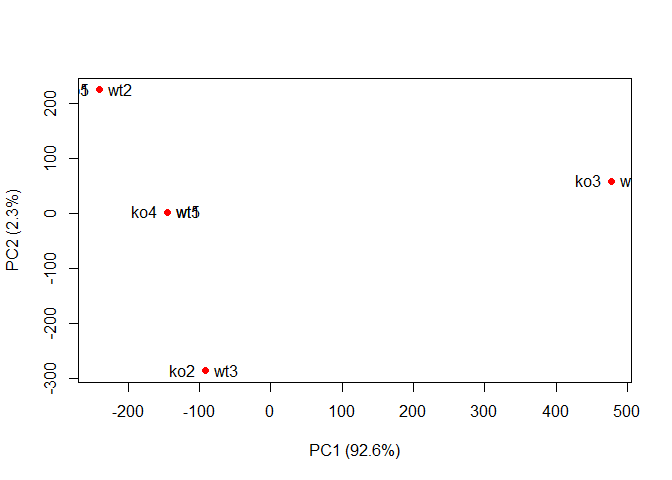
\includegraphics{Class09_files/figure-latex/unnamed-chunk-36-1.pdf}

``average''

\begin{Shaded}
\begin{Highlighting}[]
\FunctionTok{plot}\NormalTok{(}\FunctionTok{hclust}\NormalTok{(data.dist, }\AttributeTok{method =} \StringTok{"average"}\NormalTok{))}
\end{Highlighting}
\end{Shaded}

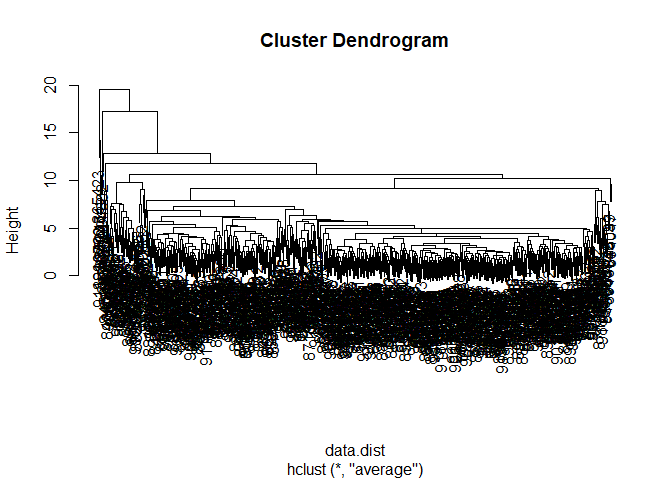
\includegraphics{Class09_files/figure-latex/unnamed-chunk-37-1.pdf}

``single''

\begin{Shaded}
\begin{Highlighting}[]
\FunctionTok{plot}\NormalTok{(}\FunctionTok{hclust}\NormalTok{(data.dist, }\AttributeTok{method =} \StringTok{"single"}\NormalTok{))}
\end{Highlighting}
\end{Shaded}

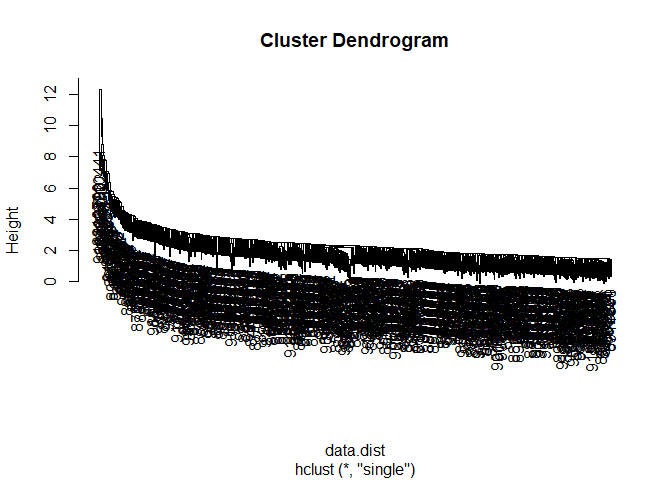
\includegraphics{Class09_files/figure-latex/unnamed-chunk-38-1.pdf}
``ward.D2''

\begin{Shaded}
\begin{Highlighting}[]
\FunctionTok{plot}\NormalTok{(}\FunctionTok{hclust}\NormalTok{(data.dist, }\AttributeTok{method =} \StringTok{"ward.D2"}\NormalTok{))}
\end{Highlighting}
\end{Shaded}

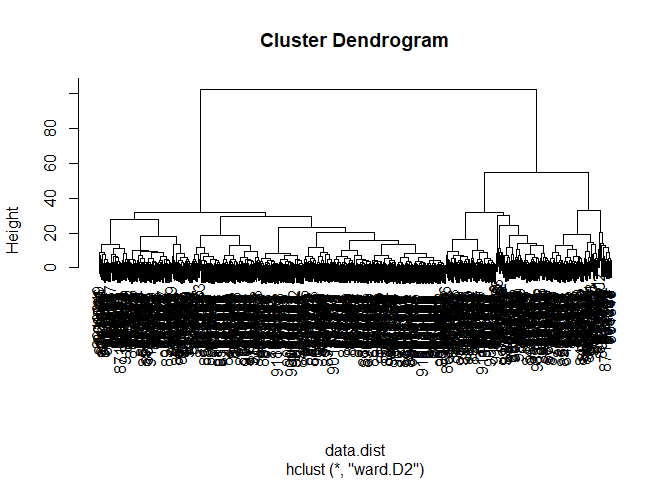
\includegraphics{Class09_files/figure-latex/unnamed-chunk-39-1.pdf} My
favorite method was ward.D2 because it was the easiest to read. The
symmetry of the plot made the larger clusters much easier to see.
Additionally, all branches ended in the same place on a horizontal line
which makes more conceptual sense to me.

\hypertarget{k-means-clustering}{%
\subsection{K-means Clustering}\label{k-means-clustering}}

\begin{Shaded}
\begin{Highlighting}[]
\NormalTok{data.scaled }\OtherTok{\textless{}{-}} \FunctionTok{scale}\NormalTok{(wisc.data)}
\NormalTok{wisc.km }\OtherTok{\textless{}{-}} \FunctionTok{kmeans}\NormalTok{(data.scaled, }\AttributeTok{centers =} \DecValTok{2}\NormalTok{, }\AttributeTok{nstart =} \DecValTok{20}\NormalTok{)}
\end{Highlighting}
\end{Shaded}

\begin{Shaded}
\begin{Highlighting}[]
\FunctionTok{table}\NormalTok{(wisc.km}\SpecialCharTok{$}\NormalTok{cluster, diagnosis)}
\end{Highlighting}
\end{Shaded}

\begin{verbatim}
##    diagnosis
##       B   M
##   1 343  37
##   2  14 175
\end{verbatim}

\begin{quote}
Q14. How well does k-means separate the two diagnoses? How does it
compare to your hclust results?
\end{quote}

\begin{Shaded}
\begin{Highlighting}[]
\FunctionTok{table}\NormalTok{(wisc.hclust.clusters, wisc.km}\SpecialCharTok{$}\NormalTok{cluster)}
\end{Highlighting}
\end{Shaded}

\begin{verbatim}
##                     
## wisc.hclust.clusters   1   2
##                    1  17 160
##                    2   0   7
##                    3 363  20
##                    4   0   2
\end{verbatim}

The k means model groups the individuals into two clear groups that can
be associated with B or M. This is fewer groups than in the hcluster
model that makes the grouping easier to understand. In general though,
the two methods corroborate with each other.

\hypertarget{combining-methods}{%
\subsection{Combining Methods}\label{combining-methods}}

Does PCA improve or degrade the performance of hierarchical clustering?

\begin{Shaded}
\begin{Highlighting}[]
\NormalTok{wisc.pr.hclust }\OtherTok{\textless{}{-}} \FunctionTok{hclust}\NormalTok{(}\FunctionTok{dist}\NormalTok{(wisc.pr}\SpecialCharTok{$}\NormalTok{x[,}\DecValTok{1}\SpecialCharTok{:}\DecValTok{7}\NormalTok{]), }\AttributeTok{method =} \StringTok{"ward.D2"}\NormalTok{)}
\FunctionTok{plot}\NormalTok{(wisc.pr.hclust)}
\end{Highlighting}
\end{Shaded}

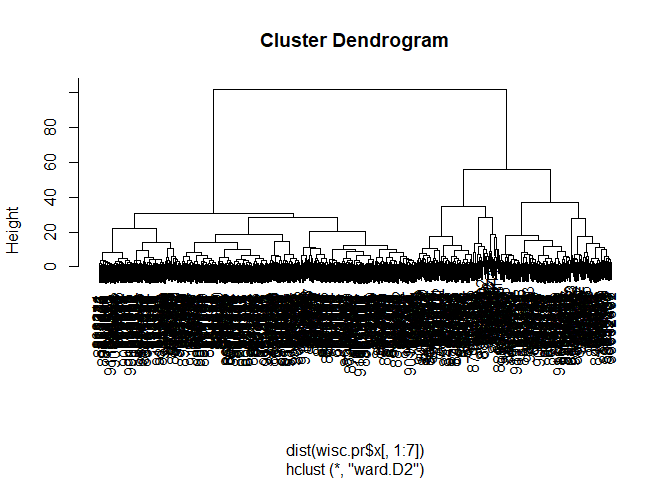
\includegraphics{Class09_files/figure-latex/unnamed-chunk-43-1.pdf}

Are these two main branches representative of malignant and benign
tumors? Can cut using h = 80 or k = 2

\begin{Shaded}
\begin{Highlighting}[]
\NormalTok{grps }\OtherTok{\textless{}{-}} \FunctionTok{cutree}\NormalTok{(wisc.pr.hclust, }\AttributeTok{k =} \DecValTok{2}\NormalTok{)}
\FunctionTok{table}\NormalTok{(grps)}
\end{Highlighting}
\end{Shaded}

\begin{verbatim}
## grps
##   1   2 
## 216 353
\end{verbatim}

\begin{Shaded}
\begin{Highlighting}[]
\FunctionTok{table}\NormalTok{(grps, diagnosis)}
\end{Highlighting}
\end{Shaded}

\begin{verbatim}
##     diagnosis
## grps   B   M
##    1  28 188
##    2 329  24
\end{verbatim}

\begin{Shaded}
\begin{Highlighting}[]
\FunctionTok{plot}\NormalTok{(wisc.pr}\SpecialCharTok{$}\NormalTok{x[, }\DecValTok{1}\SpecialCharTok{:}\DecValTok{2}\NormalTok{], }\AttributeTok{col =}\NormalTok{ grps)}
\end{Highlighting}
\end{Shaded}

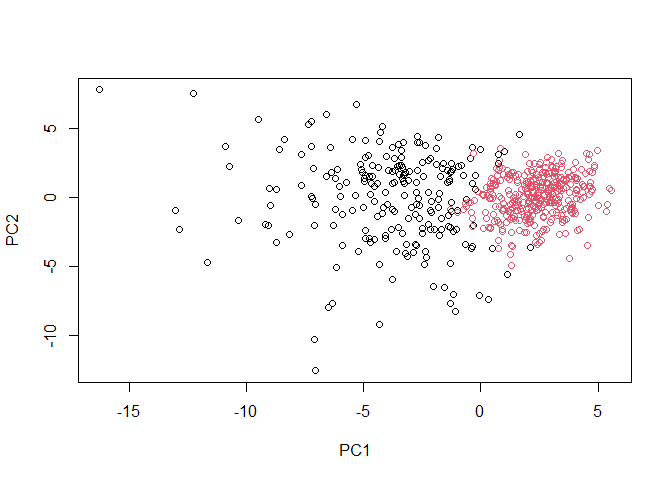
\includegraphics{Class09_files/figure-latex/unnamed-chunk-46-1.pdf}

\begin{Shaded}
\begin{Highlighting}[]
\FunctionTok{plot}\NormalTok{(wisc.pr}\SpecialCharTok{$}\NormalTok{x[, }\DecValTok{1}\SpecialCharTok{:}\DecValTok{2}\NormalTok{], }\AttributeTok{col =}\NormalTok{ diagnosis)}
\end{Highlighting}
\end{Shaded}

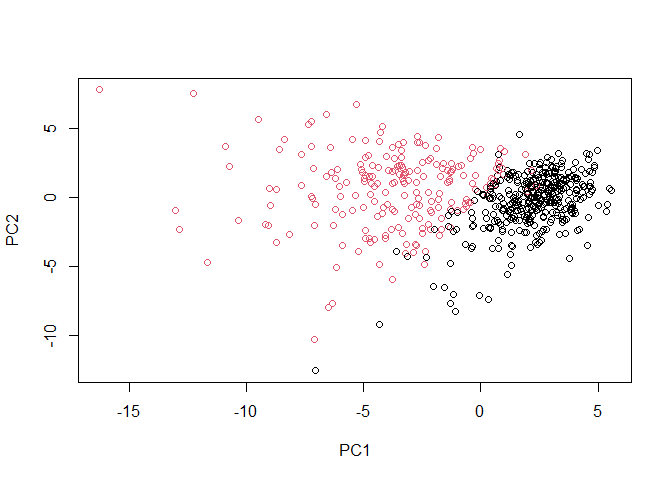
\includegraphics{Class09_files/figure-latex/unnamed-chunk-47-1.pdf} To
switch the colors so they are less confusing, turn grps into a factor
and reorder the levels

\begin{Shaded}
\begin{Highlighting}[]
\NormalTok{g }\OtherTok{\textless{}{-}} \FunctionTok{as.factor}\NormalTok{(grps)}
\FunctionTok{levels}\NormalTok{(g)}
\end{Highlighting}
\end{Shaded}

\begin{verbatim}
## [1] "1" "2"
\end{verbatim}

\begin{Shaded}
\begin{Highlighting}[]
\NormalTok{g }\OtherTok{\textless{}{-}} \FunctionTok{relevel}\NormalTok{(g,}\DecValTok{2}\NormalTok{)}
\FunctionTok{levels}\NormalTok{(g)}
\end{Highlighting}
\end{Shaded}

\begin{verbatim}
## [1] "2" "1"
\end{verbatim}

Try the plot again

\begin{Shaded}
\begin{Highlighting}[]
\FunctionTok{plot}\NormalTok{(wisc.pr}\SpecialCharTok{$}\NormalTok{x[, }\DecValTok{1}\SpecialCharTok{:}\DecValTok{2}\NormalTok{], }\AttributeTok{col =}\NormalTok{ g)}
\end{Highlighting}
\end{Shaded}

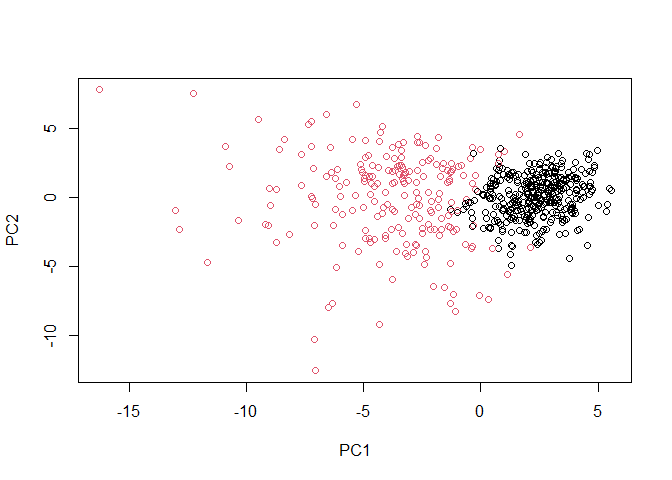
\includegraphics{Class09_files/figure-latex/unnamed-chunk-50-1.pdf}
\textgreater{} Q15. How well does the newly created model with four
clusters separate out the two diagnoses?

\begin{Shaded}
\begin{Highlighting}[]
\NormalTok{wisc.pr.hclust.clusters }\OtherTok{\textless{}{-}} \FunctionTok{cutree}\NormalTok{(wisc.pr.hclust, }\AttributeTok{k =} \DecValTok{2}\NormalTok{)}
\end{Highlighting}
\end{Shaded}

\begin{Shaded}
\begin{Highlighting}[]
\FunctionTok{table}\NormalTok{(wisc.pr.hclust.clusters, diagnosis)}
\end{Highlighting}
\end{Shaded}

\begin{verbatim}
##                        diagnosis
## wisc.pr.hclust.clusters   B   M
##                       1  28 188
##                       2 329  24
\end{verbatim}

This new combined model does a better job separating the individuals
because there are two clear groups, one associated with both B and M.
Having four clusters in the previous hclust model was more confusing
considering there are only two possible diagnoses.

\begin{quote}
Q16. How well do the k-means and hierarchical clustering models you
created in previous sections (i.e.~before PCA) do in terms of separating
the diagnoses? Again, use the table() function to compare the output of
each model (wisc.km\$cluster and wisc.hclust.clusters) with the vector
containing the actual diagnoses.
\end{quote}

\begin{Shaded}
\begin{Highlighting}[]
\FunctionTok{table}\NormalTok{(wisc.km}\SpecialCharTok{$}\NormalTok{cluster, diagnosis)}
\end{Highlighting}
\end{Shaded}

\begin{verbatim}
##    diagnosis
##       B   M
##   1 343  37
##   2  14 175
\end{verbatim}

\begin{Shaded}
\begin{Highlighting}[]
\FunctionTok{table}\NormalTok{(wisc.hclust.clusters, diagnosis)}
\end{Highlighting}
\end{Shaded}

\begin{verbatim}
##                     diagnosis
## wisc.hclust.clusters   B   M
##                    1  12 165
##                    2   2   5
##                    3 343  40
##                    4   0   2
\end{verbatim}

The k means model is more similar to the actual diagnoses because there
are only two groups whereas the hcluster model has two extra groups that
have fewer individuals and therefore are harder to confidently associate
with either B or M. Overall, the two clusterings seem to be very
similar, the two main B and M groups are only different by \textless10
individuals.

\hypertarget{sensitivity-and-specificity}{%
\subsection{Sensitivity and
Specificity}\label{sensitivity-and-specificity}}

\textbf{Sensitivity} : test's ability to correctly detect ill patients
with the condition. In this case, the total number of samples in a
cluster identified as M divided by the number of known M or TP/(TP+FN)
\textbf{Specificity} : test's ability to correctly reject healthy
patients without the condition. In this case, number of samples in a
cluster identified as B divided by the number of true B or TN/(TN+FP)
Can also look at \textbf{accuracy} = \#correct / total

\begin{Shaded}
\begin{Highlighting}[]
\CommentTok{\# for pr hclust combo}
\NormalTok{(}\DecValTok{165} \SpecialCharTok{+} \DecValTok{351}\NormalTok{)}\SpecialCharTok{/}\FunctionTok{nrow}\NormalTok{(wisc.data)}
\end{Highlighting}
\end{Shaded}

\begin{verbatim}
## [1] 0.9068541
\end{verbatim}

\begin{quote}
Q17. Which of your analysis procedures resulted in a clustering model
with the best specificity? How about sensitivity?
\end{quote}

\begin{Shaded}
\begin{Highlighting}[]
\NormalTok{hclust.sens }\OtherTok{\textless{}{-}}\NormalTok{ (}\DecValTok{165}\SpecialCharTok{+}\DecValTok{5}\SpecialCharTok{+}\DecValTok{2}\NormalTok{)}\SpecialCharTok{/}\NormalTok{(}\DecValTok{165}\SpecialCharTok{+}\DecValTok{5}\SpecialCharTok{+}\DecValTok{2}\SpecialCharTok{+}\DecValTok{40}\NormalTok{)}
\NormalTok{hclust.spec }\OtherTok{\textless{}{-}} \DecValTok{343}\SpecialCharTok{/}\NormalTok{(}\DecValTok{343}\SpecialCharTok{+}\DecValTok{12}\SpecialCharTok{+}\DecValTok{2}\NormalTok{)}
\NormalTok{hclust.pr.sens }\OtherTok{\textless{}{-}} \DecValTok{188}\SpecialCharTok{/}\NormalTok{(}\DecValTok{188}\SpecialCharTok{+}\DecValTok{24}\NormalTok{)}
\NormalTok{hclust.pr.spec }\OtherTok{\textless{}{-}} \DecValTok{329}\SpecialCharTok{/}\NormalTok{(}\DecValTok{329}\SpecialCharTok{+}\DecValTok{28}\NormalTok{)}
\NormalTok{kmeans.sens }\OtherTok{\textless{}{-}} \DecValTok{175}\SpecialCharTok{/}\NormalTok{(}\DecValTok{175}\SpecialCharTok{+}\DecValTok{37}\NormalTok{)}
\NormalTok{kmeans.spec }\OtherTok{\textless{}{-}} \DecValTok{343}\SpecialCharTok{/}\NormalTok{(}\DecValTok{343}\SpecialCharTok{+}\DecValTok{14}\NormalTok{)}
\end{Highlighting}
\end{Shaded}

\begin{Shaded}
\begin{Highlighting}[]
\NormalTok{hclust.sens}
\end{Highlighting}
\end{Shaded}

\begin{verbatim}
## [1] 0.8113208
\end{verbatim}

\begin{Shaded}
\begin{Highlighting}[]
\NormalTok{hclust.spec}
\end{Highlighting}
\end{Shaded}

\begin{verbatim}
## [1] 0.9607843
\end{verbatim}

\begin{Shaded}
\begin{Highlighting}[]
\NormalTok{hclust.pr.sens}
\end{Highlighting}
\end{Shaded}

\begin{verbatim}
## [1] 0.8867925
\end{verbatim}

\begin{Shaded}
\begin{Highlighting}[]
\NormalTok{hclust.pr.spec}
\end{Highlighting}
\end{Shaded}

\begin{verbatim}
## [1] 0.9215686
\end{verbatim}

\begin{Shaded}
\begin{Highlighting}[]
\NormalTok{kmeans.sens}
\end{Highlighting}
\end{Shaded}

\begin{verbatim}
## [1] 0.8254717
\end{verbatim}

\begin{Shaded}
\begin{Highlighting}[]
\NormalTok{kmeans.spec}
\end{Highlighting}
\end{Shaded}

\begin{verbatim}
## [1] 0.9607843
\end{verbatim}

\textbf{Sensitivity}: hclust/PCA \textgreater{} K-means \textgreater{}
hclust

\textbf{Specificity}: hclust = K-means \textgreater{} hclust/PCA

\hypertarget{prediction}{%
\subsection{Prediction}\label{prediction}}

Take our previous PCA model and apply it to new cancer cell data

\begin{Shaded}
\begin{Highlighting}[]
\NormalTok{url }\OtherTok{\textless{}{-}} \StringTok{"https://tinyurl.com/new{-}samples{-}CSV"}
\NormalTok{new }\OtherTok{\textless{}{-}} \FunctionTok{read.csv}\NormalTok{(url)}
\NormalTok{npc }\OtherTok{\textless{}{-}} \FunctionTok{predict}\NormalTok{(wisc.pr, }\AttributeTok{newdata=}\NormalTok{new)}
\NormalTok{npc}
\end{Highlighting}
\end{Shaded}

\begin{verbatim}
##            PC1       PC2        PC3        PC4       PC5        PC6        PC7
## [1,]  2.576616 -3.135913  1.3990492 -0.7631950  2.781648 -0.8150185 -0.3959098
## [2,] -4.754928 -3.009033 -0.1660946 -0.6052952 -1.140698 -1.2189945  0.8193031
##             PC8       PC9       PC10      PC11      PC12      PC13     PC14
## [1,] -0.2307350 0.1029569 -0.9272861 0.3411457  0.375921 0.1610764 1.187882
## [2,] -0.3307423 0.5281896 -0.4855301 0.7173233 -1.185917 0.5893856 0.303029
##           PC15       PC16        PC17        PC18        PC19       PC20
## [1,] 0.3216974 -0.1743616 -0.07875393 -0.11207028 -0.08802955 -0.2495216
## [2,] 0.1299153  0.1448061 -0.40509706  0.06565549  0.25591230 -0.4289500
##            PC21       PC22       PC23       PC24        PC25         PC26
## [1,]  0.1228233 0.09358453 0.08347651  0.1223396  0.02124121  0.078884581
## [2,] -0.1224776 0.01732146 0.06316631 -0.2338618 -0.20755948 -0.009833238
##              PC27        PC28         PC29         PC30
## [1,]  0.220199544 -0.02946023 -0.015620933  0.005269029
## [2,] -0.001134152  0.09638361  0.002795349 -0.019015820
\end{verbatim}

Add these samples to our PCA plot

\begin{Shaded}
\begin{Highlighting}[]
\FunctionTok{plot}\NormalTok{(wisc.pr}\SpecialCharTok{$}\NormalTok{x[,}\DecValTok{1}\SpecialCharTok{:}\DecValTok{2}\NormalTok{], }\AttributeTok{col =}\NormalTok{ g)}
\FunctionTok{points}\NormalTok{(npc[,}\DecValTok{1}\NormalTok{], npc[,}\DecValTok{2}\NormalTok{], }\AttributeTok{col =} \StringTok{"blue"}\NormalTok{, }\AttributeTok{pch =} \DecValTok{16}\NormalTok{, }\AttributeTok{cex =} \DecValTok{3}\NormalTok{)}
\FunctionTok{text}\NormalTok{(npc[,}\DecValTok{1}\NormalTok{], npc[,}\DecValTok{2}\NormalTok{], }\FunctionTok{c}\NormalTok{(}\DecValTok{1}\NormalTok{,}\DecValTok{2}\NormalTok{), }\AttributeTok{col =} \StringTok{"white"}\NormalTok{)}
\end{Highlighting}
\end{Shaded}

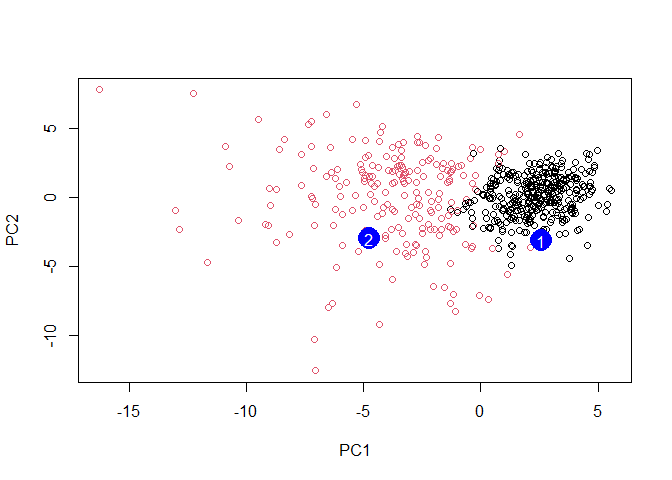
\includegraphics{Class09_files/figure-latex/unnamed-chunk-59-1.pdf}
\textgreater{} Q18. Which of these new patients should we prioritize for
follow up based on your results?

We would prioritize patient 2 because they are grouped in the malignant
group.

\end{document}
